

\documentclass{article}
\usepackage[utf8]{inputenc}
\usepackage{authblk}
\usepackage{setspace}
\usepackage[margin=1.25in]{geometry}
\usepackage{graphicx}
\graphicspath{ {./figures/} }
\usepackage{subcaption}
\usepackage{amsmath}
\usepackage{lineno}
\usepackage{datetime2}
\linenumbers



%%%%%% Bibliography %%%%%%
% Replace "sample" in the \addbibresource line below with the name of your .bib file.
\usepackage[style=ieee, 
citestyle=numeric-comp,
sorting=none]{biblatex}
\addbibresource{sample.bib}

%%%%%% Title %%%%%%
% Full titles can be a maximum of 200 characters, including spaces. 
% Title Format: Use title case, capitalizing the first letter of each word, except for certain small words, such as articles and short prepositions
\title{Machine Learning-Based Mood Classification in Music }

%%%%%% Authors %%%%%%
% Authors should be listed in order of contribution to the paper, by first name, then middle initial (if any), followed by last name.
% Authors should be listed in the order in which they will appear in the published version if the manuscript is accepted. 
% Use an asterisk (*) to identify the corresponding author, and be sure to include that person’s e-mail address. Use symbols (in this order: †, ‡, §, ||, ¶, #, ††, ‡‡, etc.) for author notes, such as present addresses, “These authors contributed equally to this work” notations, and similar information.
% You can include group authors, but please include a list of the actual authors (the group members) in the Supplementary Materials.
\author{Weiting Lin, Yuxi Jiang, Hungta Chen, Jaehyeon Park}
\date{\today}


%%%%%% Affiliations %%%%%%
% \affil[1]{Department of Physics, A University, City, Country.}
% \affil[2]{Department of Astronomy, B University, City, Country.}
% \affil[*]{Corresponding author. Email: email@email.com}
% \affil[$\dag$]{These authors contributed equally to this work.}

%%%%%% Date %%%%%%
% Date is optional
\date{}

%%%%%% Spacing %%%%%%
% Use paragraph spacing of 1.5 or 2 (for double spacing, use command \doublespacing)
\onehalfspacing

\begin{document}

\maketitle

%%%%%% Abstract %%%%%%
\begin{abstract}
In this paper, our goal is to classify music based on four moods. The rest of the paper is organized as follows: we will first use the API to fetch data from Spotify and perform thorough data preprocessing, including data normalization, outlier removal, and data denoising. After cleaning the data, we will leverage several machine learning methods, such as random forest and deep neural networks, to build models for data classification
% \begin{itemize}
%     \item An opening sentence that states the question/problem addressed by the research AND
%     \item Enough background content to give context to the study AND
%     \item A brief statement of primary results AND
%     \item A short concluding sentence.
% \end{itemize} 
\end{abstract}

%%%%%% Main Text %%%%%%

\section{Introduction}
Nowadays, music has become a critical part of our lives, and research indicated that it can be classified based on mood. Many music platforms already utilize mood classification to personalize playlists for their clients. This demonstrates the practicality and relevance of mood classification in the market. Inspired by these developments, we are driven by exploring the potential of efficiently categorizing music using machine learning techniques.

\section{Data description}
To achieve our goal of efficient music categorization based on mood, we begin by acquiring data through the Spotify API. Our aim is to identify music playlists that correspond to four distinct mood types: anger, relaxation(chill), happiness, and depression. The selection of these mood types is influenced by prior research such as "Music Mood Classification" by Michael Nuzzolo and "What music makes us feel: At least 13 dimensions organize subjective experiences associated with music across different cultures" by Alan S. Cowen.\\ 

However, it is important to acknowledge that playlist classifications can sometimes be subjective, with some playlists containing music from multiple mood types. Hence, we assume that each playlist is objective and that all the music within a given playlist belongs to the same mood type. We plan to collect 1000 songs for each mood category in this project and carefully label them accordingly.\\

There are two types of features that we will use in this project, the first type is continuous features and the second type is categorical features. We will have 9 continuous features (danceability, energy, loudness, speechiness, acousticness, instrumentalness, liveness, valence, tempo) and 3 categorical features (key, mode, time signature) leveraged in this project, and the description of features will be placed in the features description link of reference. 
We aim to construct three distinct datasets for our analysis. These datasets will consist of:

\begin{enumerate}
    \begin{itemize}
        \item The first dataset will include only continuous features.
        \item The second dataset will encompass all available features, regardless of their type (continuous or categorical).
        \item The third dataset will focus on including only the most relevant and significant features.
    \end{itemize}
\end{enumerate}

By creating these diverse datasets, we can explore the impact and effectiveness of different feature subsets on our analysis.

\begin{figure}[!htbp]
\centering
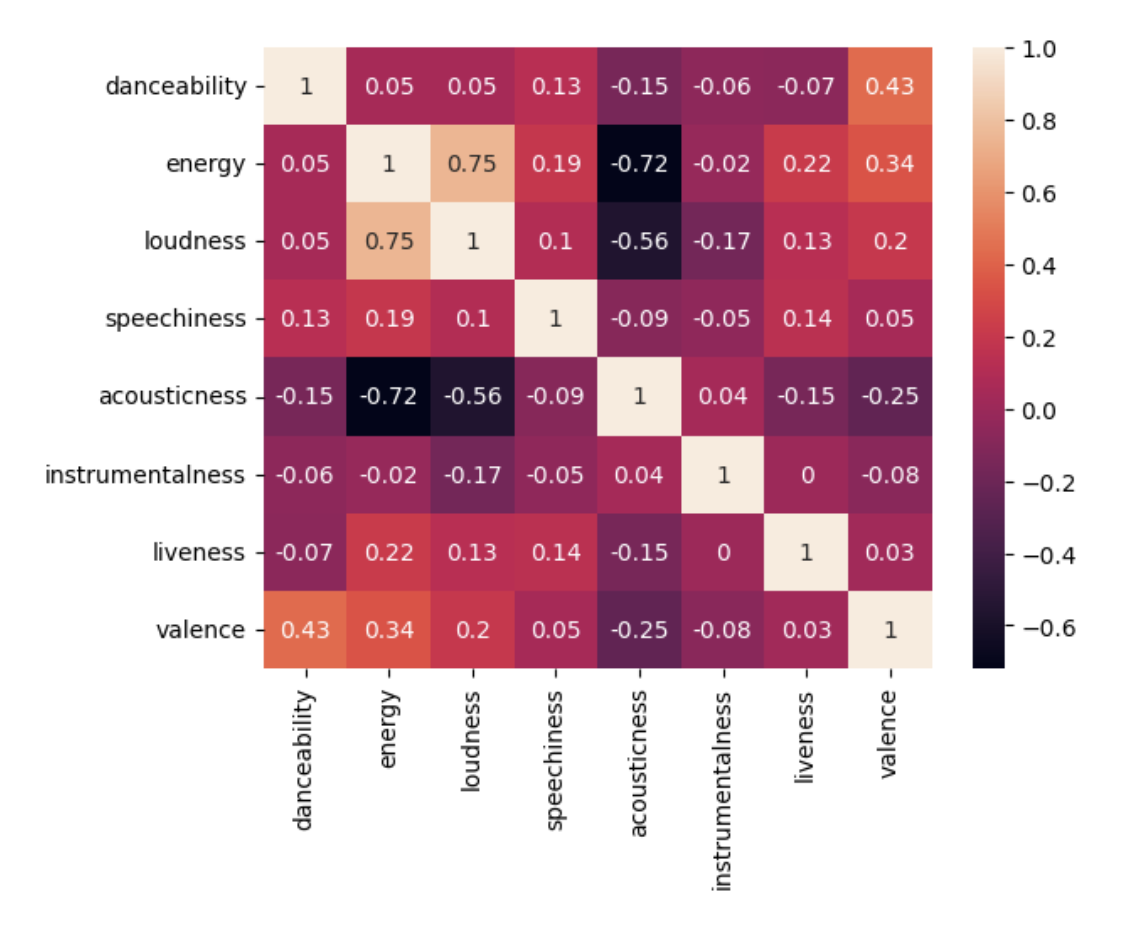
\includegraphics[scale=0.6]{heatmap.png}
\caption{correlation between continuous variables}
\end{figure}

We will determine third dataset based on the heatmap, we would like to select danceability, energy, loudness, acousticness, valence as the relative critical features due to the higher corresponding correlation.
\newpage
\subsection{Exploratory Data Analysis}
\begin{figure}[!htb]
   \begin{minipage}{0.48\textwidth}
     \centering
     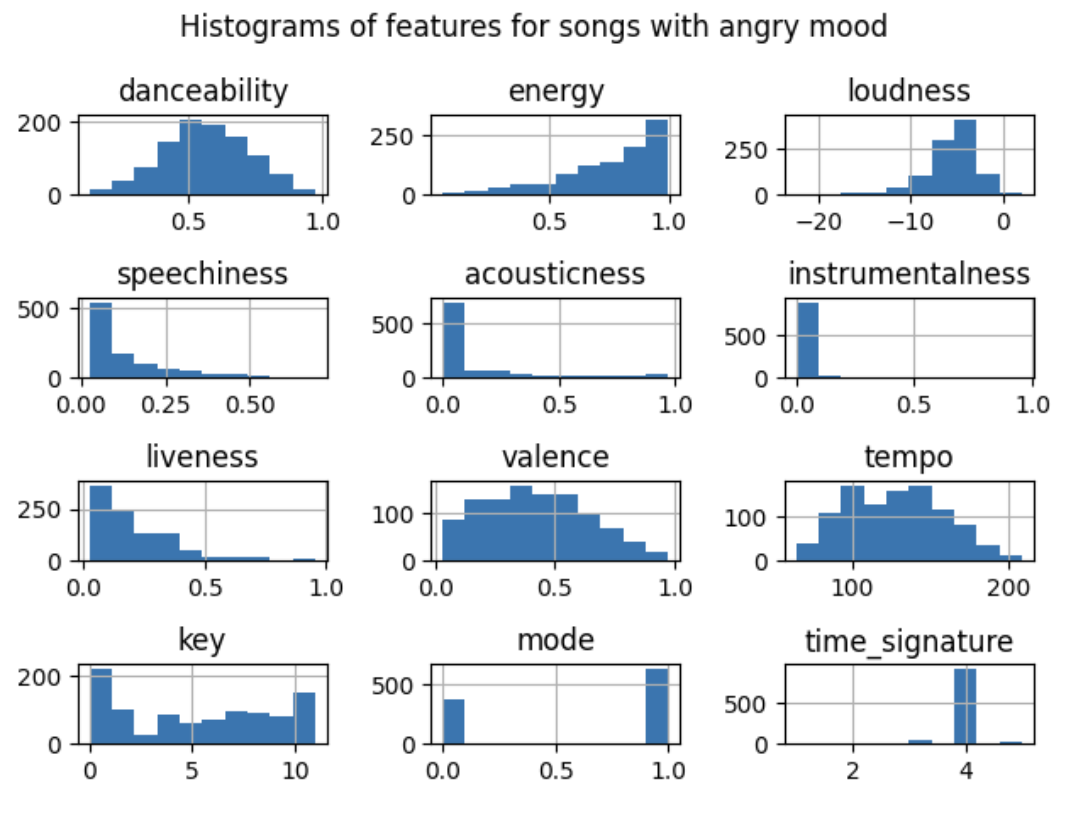
\includegraphics[scale=0.4]{angry .png}
     \caption{Features histogram in angry songs}\label{Fig:Data1}
   \end{minipage}\hfill
   \begin{minipage}{0.48\textwidth}
     \centering
     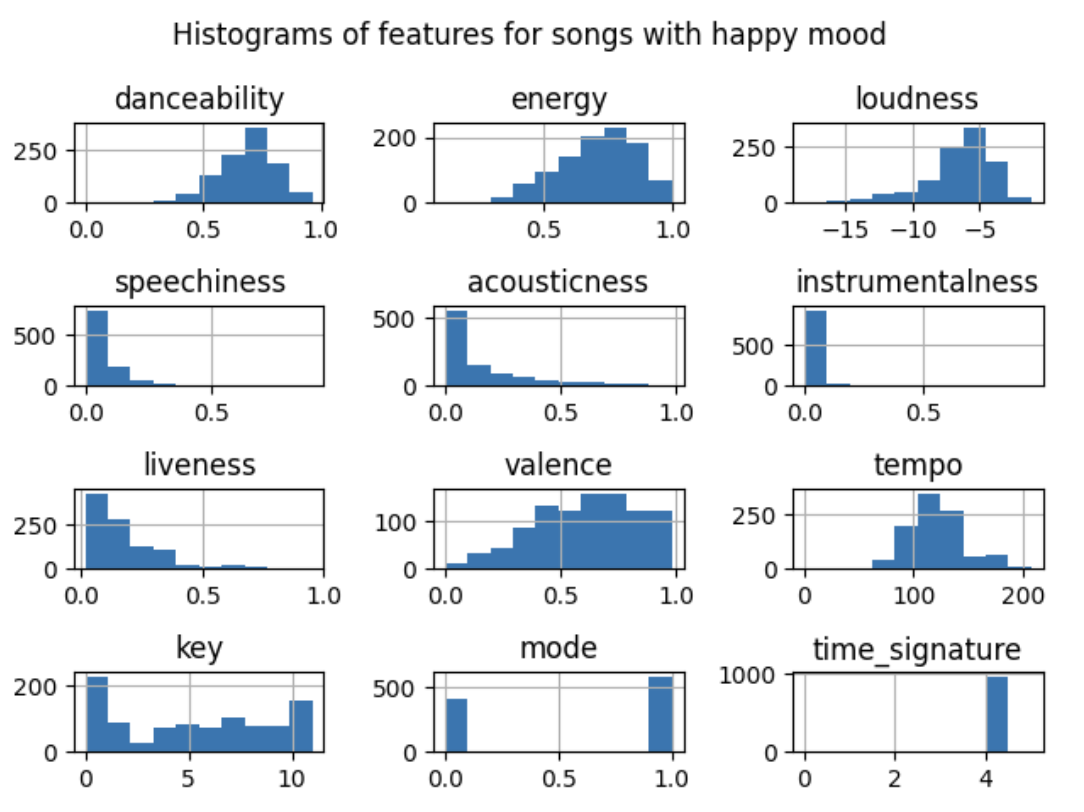
\includegraphics[scale=0.4]{happy.png}
     \caption{Features histogram in happy songs}\label{Fig:Data2}
   \end{minipage}
\end{figure}

We found that the energy feature in angry songs receives a higher score, which is reasonable considering that this genre of music is often characterized by its emotional intensity.Happy songs exhibit a tendency for the valence feature to approach a value close to 1, signifying their ability to convey a strong sense of musical positivity. Furthermore, happy songs tend to have higher energy features, further contributing to their lively and upbeat nature.

\begin{figure}[!htb]
   \begin{minipage}{0.48\textwidth}
     \centering
     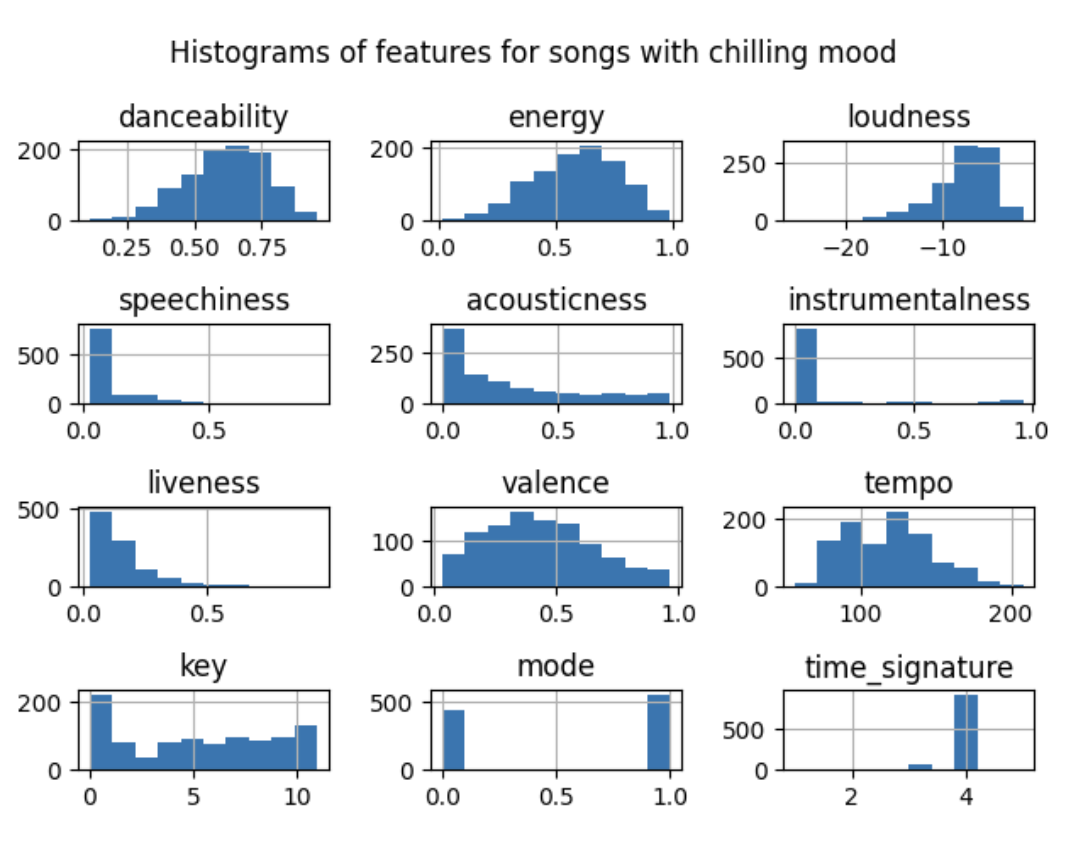
\includegraphics[scale=0.4]{ chill.png}
     \caption{Features histogram in angry songs}\label{Fig:Data1}
   \end{minipage}\hfill
   \begin{minipage}{0.48\textwidth}
     \centering
     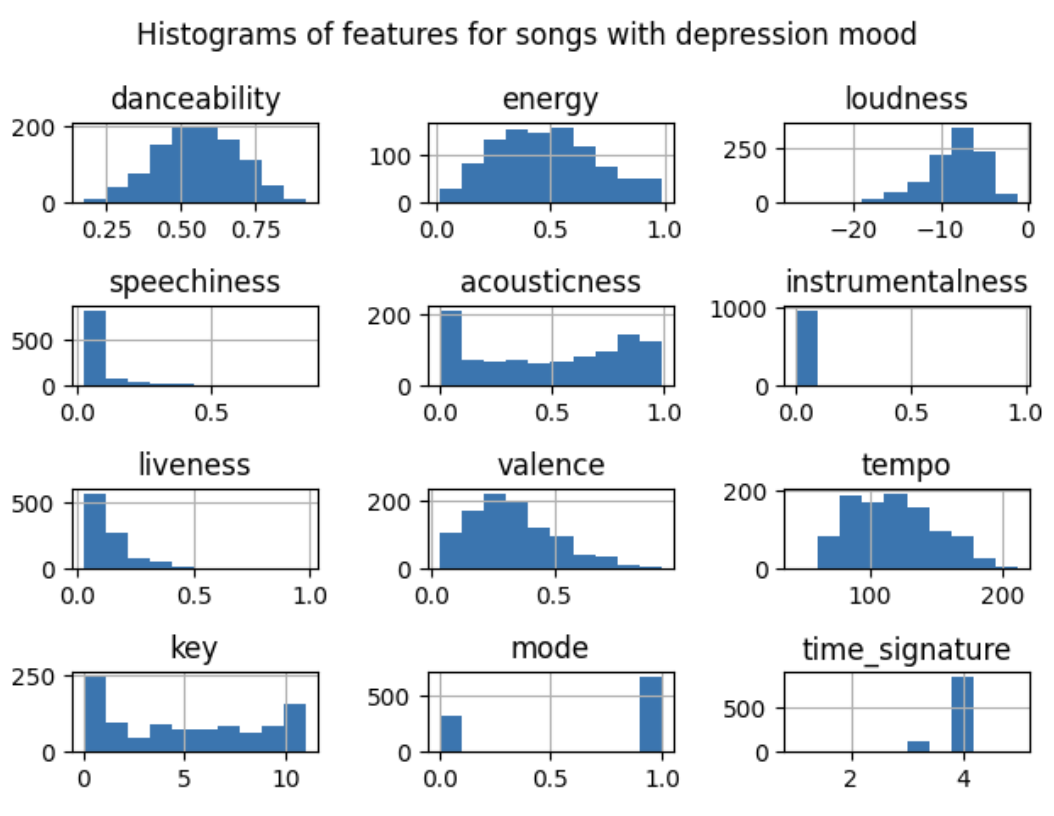
\includegraphics[scale=0.4]{despression.png}
     \caption{Features histogram in happy songs}\label{Fig:Data2}
   \end{minipage}
\end{figure}

% \begin{figure}[!htbp]
% \centering
% 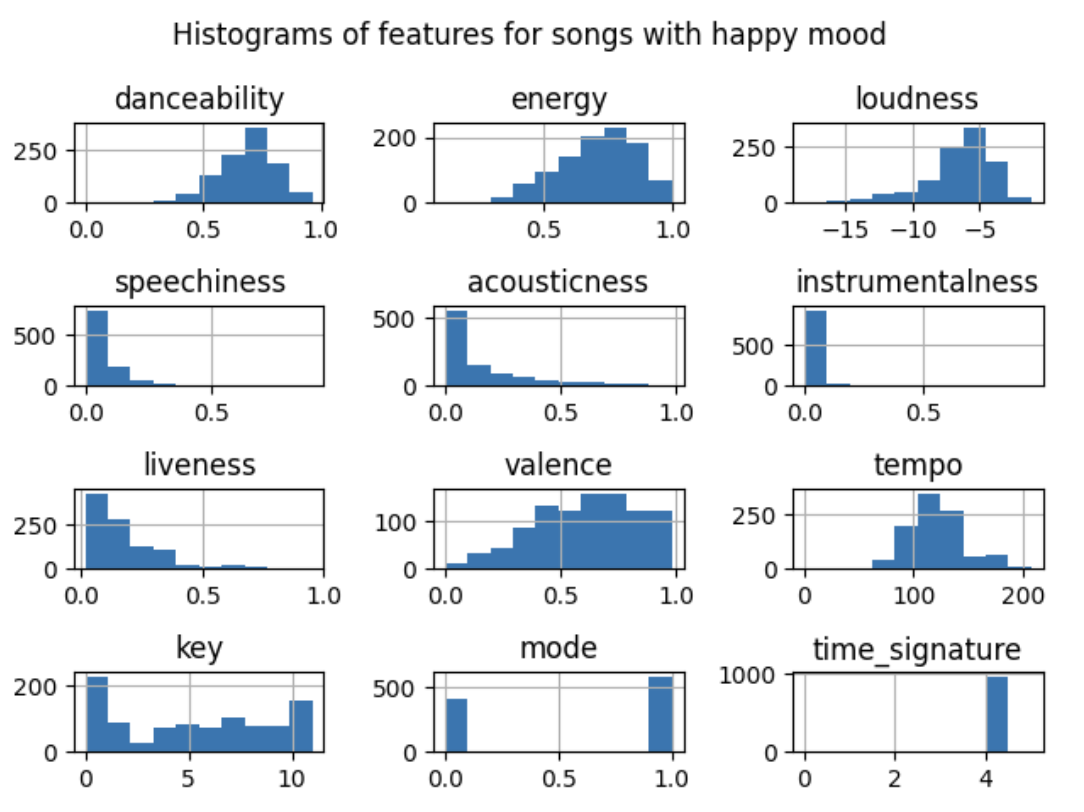
\includegraphics[scale=0.5]{happy.png}
% \caption{features histogram in happy songs}
% \end{figure}
In chill songs, which are commonly known as relaxation songs, there is a higher emphasis on the acousticness feature. This can be attributed to the fact that most chill songs predominantly consist of instruments or white noise, resulting in a greater presence of acoustic elements in the music.In depression songs, the valence, extent of positivity in the track, is opposite to the happy songs. This result is reasonable. 

\newpage
% \begin{figure}[!htbp]
% \centering
% 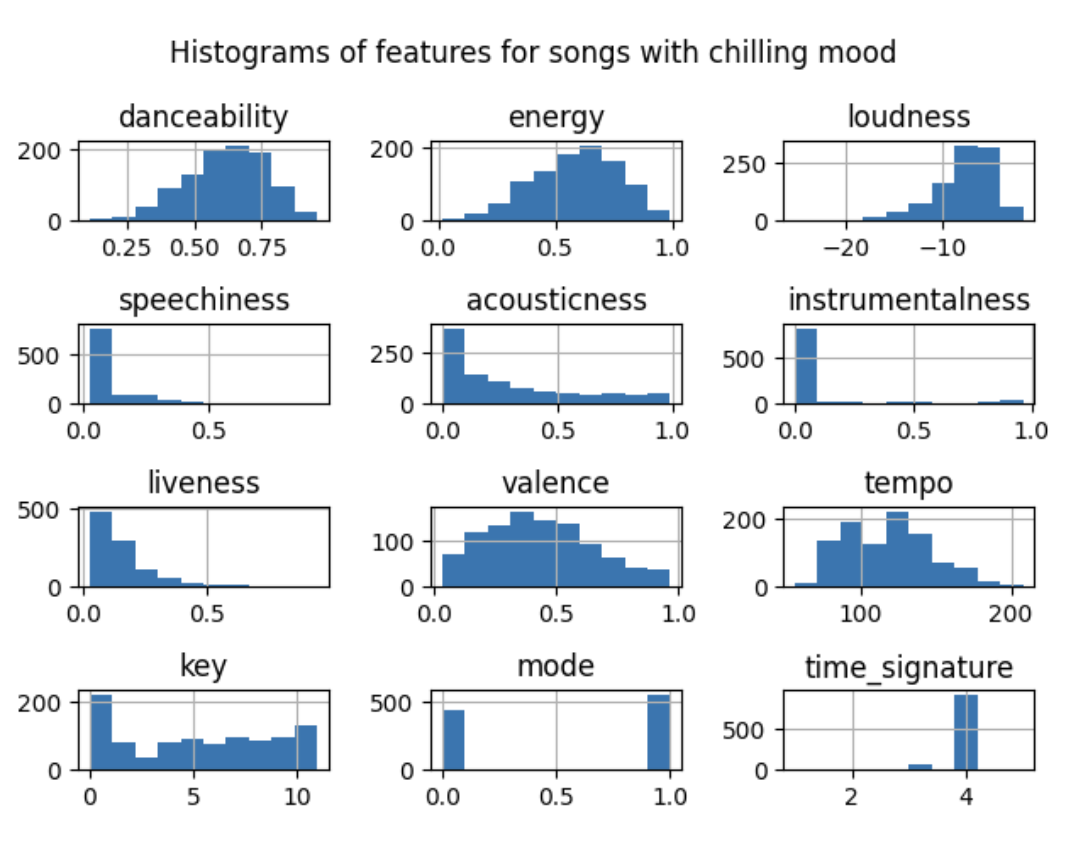
\includegraphics[scale=0.5]{chill.png}
% \caption{features histogram in chilling songs}
% \end{figure}




% \begin{figure}[!htbp]
% \centering
% 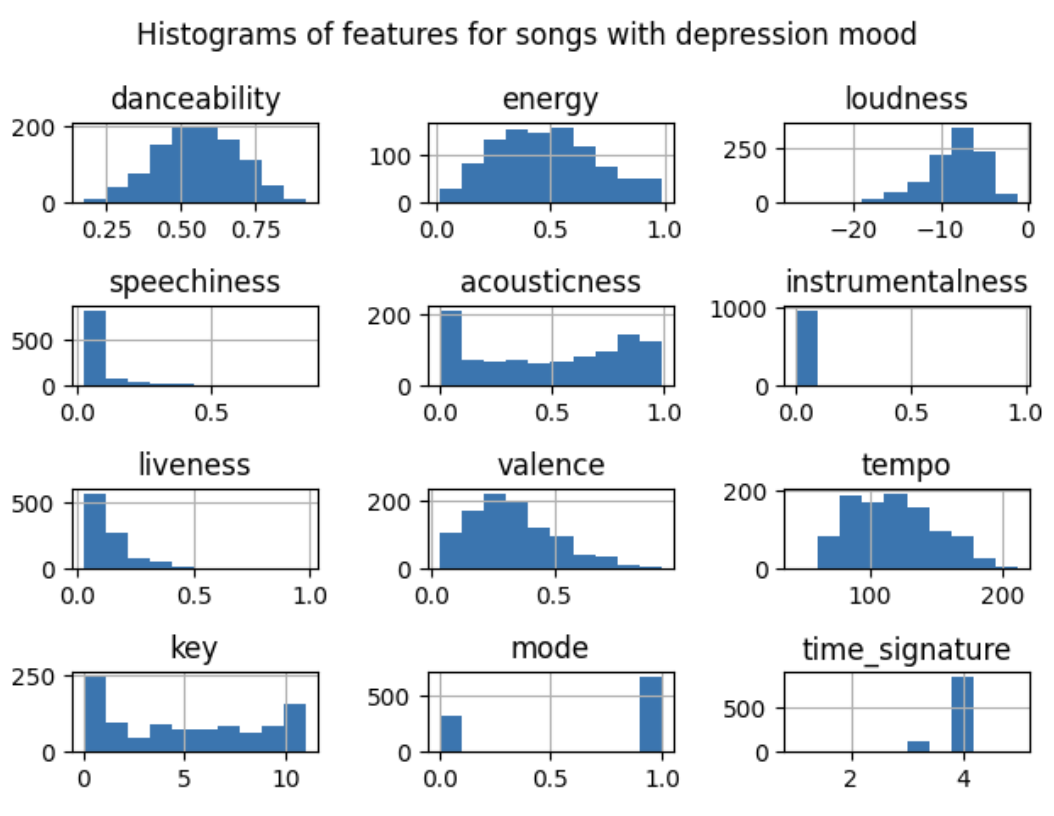
\includegraphics[scale=0.5]{despression.png}
% \caption{features histogram in depression songs}
% \end{figure}



% By undertaking this project, we aspire to contribute to the field of music mood classification. Our objective is to develop a robust and efficient system that can accurately categorize music based on mood. We believe that this system can have various applications, including personalized music recommendations, and a deeper understanding of the emotional impact of music. 



% %%%%% Citations in the text %%%%%%
% \subsection*{Citations}
% Citations of references in the text should be identified using numbers in square brackets e.g., ``as discussed by Cui \cite{Cui1}'' or ``as discussed elsewhere \cite{Cui1,Ninomiya1,Li1,Wang1,Yang1}.'' All references should be cited within the text and uncited references will be removed. 

% As an example, this template includes a ``sample.bib'' file containing the references in BibTeX.

% %%%%%% Equations %%%%%%
% \subsection*{Equations}
% Equations should be provided in a text format, rather than as an image. Equations should be numbered consecutively, in round brackets, on the right-hand side of the page by using the ``\textbackslash begin\{equation\}'' command. They should be referred to as Equation 1, etc. in the main text.

% \medskip For example, see Equation \ref{eq:1} and Equation \ref{eq:2} below.
% \begin{equation} \label{eq:1}
%     a^2 + b^2 = c^2
% \end{equation}
% \begin{equation} \label{eq:2}
% \begin{split}
% A & = \frac{\pi r^2}{2} \\
%  & = \frac{1}{2} \pi r^2
% \end{split}
% \end{equation}

% %%%%%% Figures %%%%%%
% \subsection*{Figures}
% Figures should be called out within the text and numbered in the order of their citation in the text. Every figure must have a descriptive title beginning with ``Figure [Number] …'' All figure titles should be either a phrase or a sentence; do not mix the two styles. See Figure \ref{fig:1} for example.
% \begin{figure}[h]
%     \centering
%     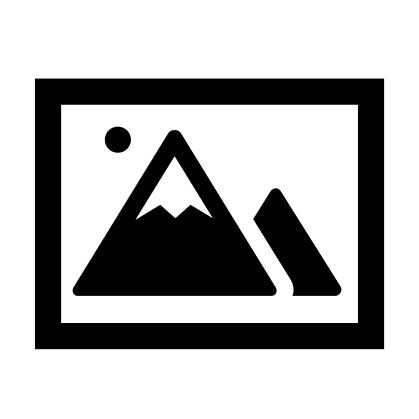
\includegraphics[width=0.5\textwidth]{fig 1}
%     \caption{This is an example figure.}
%     \label{fig:1}
% \end{figure}

% Figures should be displayed on a white background. When preparing figures, consider that they can occupy either a single column (half page width) or two columns (full page width), and should be sized accordingly.

% If a figure consists of multiple panels, they should be ordered logically and labelled with lower case roman letters (i.e., a, b, c, etc.). All labels should be explained in the legend. See Figure \ref{fig:2} for example.

% Upon acceptance, authors will be asked to provide the figures as separate electronic files. At that stage, figures should be supplied in either vector art formats (PS, EPS, FIG, AI, Visio, WMF, EMF, Word, Excel, PowerPoint, OPJ, CDR, or PDF) or bitmap formats (Photoshop, TIFF, GIF, JPEG, PNG, BMP, etc.). Bitmap (BMP) images should be of at least 300 dpi resolution, unless due to the limited resolution of a scientific instrument. If a bitmap image has labels, the image and labels should be embedded in separate layers.
% \begin{figure}[h]
%     \centering
%     \begin{subfigure}{0.4\textwidth}
%         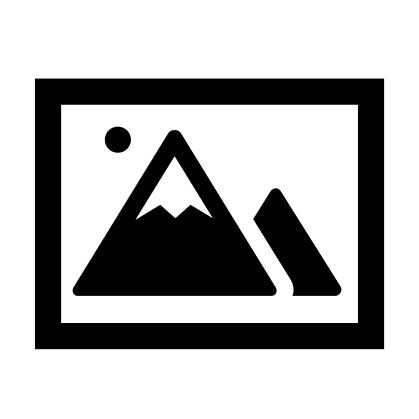
\includegraphics[width=0.9\textwidth, height=2in]{fig 1}
%         \caption{\label{fig:2a}}
%     \end{subfigure}
%     \begin{subfigure}{0.4\textwidth}
%         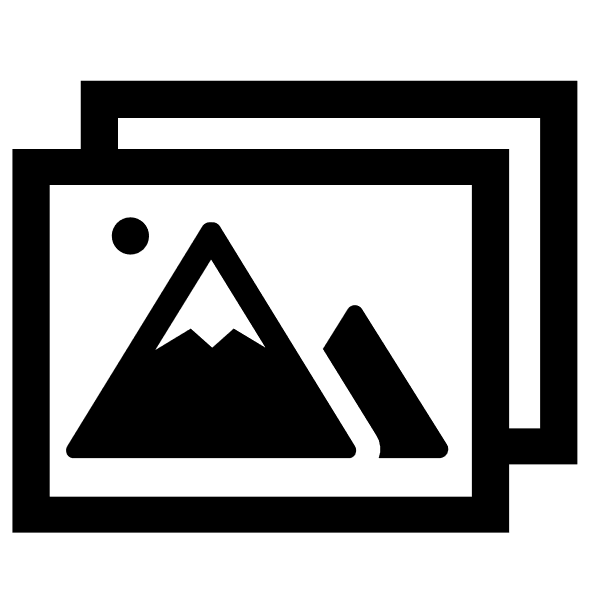
\includegraphics[width=0.9\textwidth, height=2in]{fig 2}
%         \caption{\label{fig:2b}}
%     \end{subfigure}
%     \caption{This is an example of a figure consisting of multiple panels.     (\subref{fig:2a}) This is the first panel. (\subref{fig:2b}) This is the second panel.}
%     \label{fig:2}
% \end{figure}

% %%%%%% Tables %%%%%%
% \subsection*{Tables}
% Tables should supplement, not duplicate, the text. They should be called out consecutively within the text and numbered in the order of their citation in the text. 

% Every table must have a descriptive title beginning with ``Table [Number] …'' as noted in Table \ref{tab:1}. If numerical measurements are given, the units should be included in the column heading. Every vertical column should have a heading, followed by a unit of measure (if any) in parentheses. Units should not change within a column. Vertical rules should not be used. 

% Centered headings of the body of the table can be used to break the entries into groups. Do not use footnotes in column heads; include any such details in sentence form in the table legend. Footnotes should contain information relevant to specific cells of the table; use the following symbols in order, as needed: $*, \dag, \ddag, \S, \|, \P, \#, **, \dag\dag$, etc.



% \end{table}

\section{Proposed Methods}

\subsection{Intuition}
Our proposed methods for music mood classification, which include Principal Component Analysis (PCA), Support Vector Machines (SVM) with different kernels, decision trees, random forests, Linear Discriminant Analysis (LDA), and deep neural networks, may have several advantages on this task:

\begin{enumerate}
  \item Feature Extraction with PCA: 
  
  PCA helps reduce the dimensionality of the music data while retaining the most relevant information related to mood. By effectively capturing the essential characteristics of the songs, PCA may improve the efficiency and effectiveness of the classification.
  \item Ensemble Learning with Random Forest: 
  
  Random Forest is an ensemble learning method that combines multiple decision trees to make predictions. It can handle high-dimensional data and capture complicated relationships between features. By utilizing the power of ensemble learning, we may be able to create a more robust music mood classification model that is less prone to overfitting.
  
  \item Deep Neural Networks for Capturing Complex Patterns: 
  
  Deep neural networks have demonstrated exceptional success in many domains, including audio and music processing. They excel at capturing complex patterns and extracting hierarchical representations from the data. By incorporating deep neural networks into our proposed method, we can leverage their capability to capture intricate musical features and potentially enhance the accuracy of mood classification.
\end{enumerate}

\subsection{Description of the methods}
\begin{enumerate}
  \item \textbf{Principal Component Analysis} 

  PCA is applied with a variance retention threshold of 95\% to reduce the dimensionality of the music data while preserving the most important mood-related features. The resulting transformed data is used for further analysis.
  
  \item \textbf{Support Vector Machines}

  The proposed method utilizes SVM with different kernels:
  \begin{itemize}
    \item Linear Kernel: 
    
    A linear kernel is employed to classify the music data into mood categories with a linear decision boundary.
    \item Polynomial Kernel: 
    
    The polynomial kernel is utilized to capture nonlinear relationships between features.
    \item RBF (Radial Basis Function) Kernel: 
    
    The RBF kernel is used to model complex and nonlinear decision boundaries.
    \item Sigmoid Kernel: 
    
    The sigmoid kernel is employed to capture nonlinear relationships with a sigmoid-shaped decision boundary.
\end{itemize}

Also, the OneVsOne decision function shape is utilized for multiclass classification, enabling SVM to handle multiple mood categories.
  
  \item \textbf{Decision Tree}

  The decision tree algorithm is used to partition the music data based on different features. The decision tree structure allows the model to make decisions at each internal node based on specific features, leading to the classification of music into different mood categories.

  \item \textbf{Random Forest}

  The random forest model is an ensemble learning method, combining multiple decision trees, where each tree is trained on a random subset of features. By aggregating the predictions of individual trees, the random forest produces the final prediction. This approach helps to improve the accuracy and robustness of the music mood classification by reducing overfitting and capturing complex relationships in the data.

  \item \textbf{Linear Discriminant Analysis}
  
  LDA is utilized to reduce the dimensionality of the music data while enhancing the separability between different mood categories. By finding a linear combination of features that maximizes the separation between classes, LDA contributes to improved accuracy in music mood classification.

  \item \textbf{Deep Neural Networks}
  
  We proposed a deep neural network with several hidden layers.  Our model has the following architecture: 
  \begin{itemize}
  \item Input Layer: The input layer is designed to have the same number of units as the features in the music data.

  \item  Hidden Layers: We used Multiple hidden layers with 80, 20, 20, 10, and 10 units respectively. Dropout regularization with a rate of 0.2 is applied to prevent overfitting.

  \item Output Layer: The output layer consists of 4 units, corresponding to the number of mood categories. The softmax activation function is used to generate probabilities for each category.
  \end{itemize}

  As for the activation function, ReLU function is used in the hidden layers to introduce nonlinearity and capture complex patterns in the music data.

  Also, we explore various optimizers, including Adadelta, Adagrad, Adam, RMSprop, and SGD, to train the DNN model for better performance and convergence of the model. The model is trained using categorical cross-entropy loss and accuracy as the evaluation metric.


\end{enumerate}
\begin{figure}[!htbp]
\centering
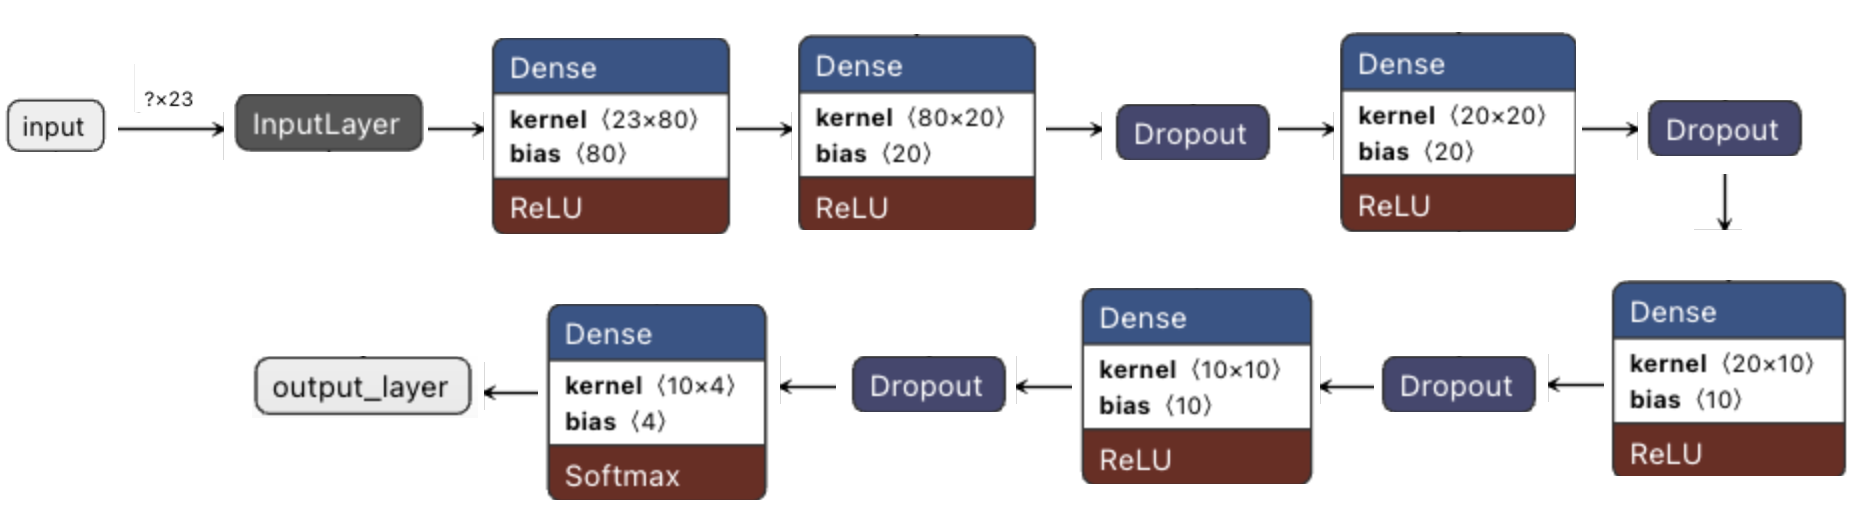
\includegraphics[scale=0.5]{model.png}
\caption{Architecture of DNN model}
\end{figure}

% \begin{figure}[h]
% \begin{subfigure}{0.5\textwidth}
% \hspace*{3cm}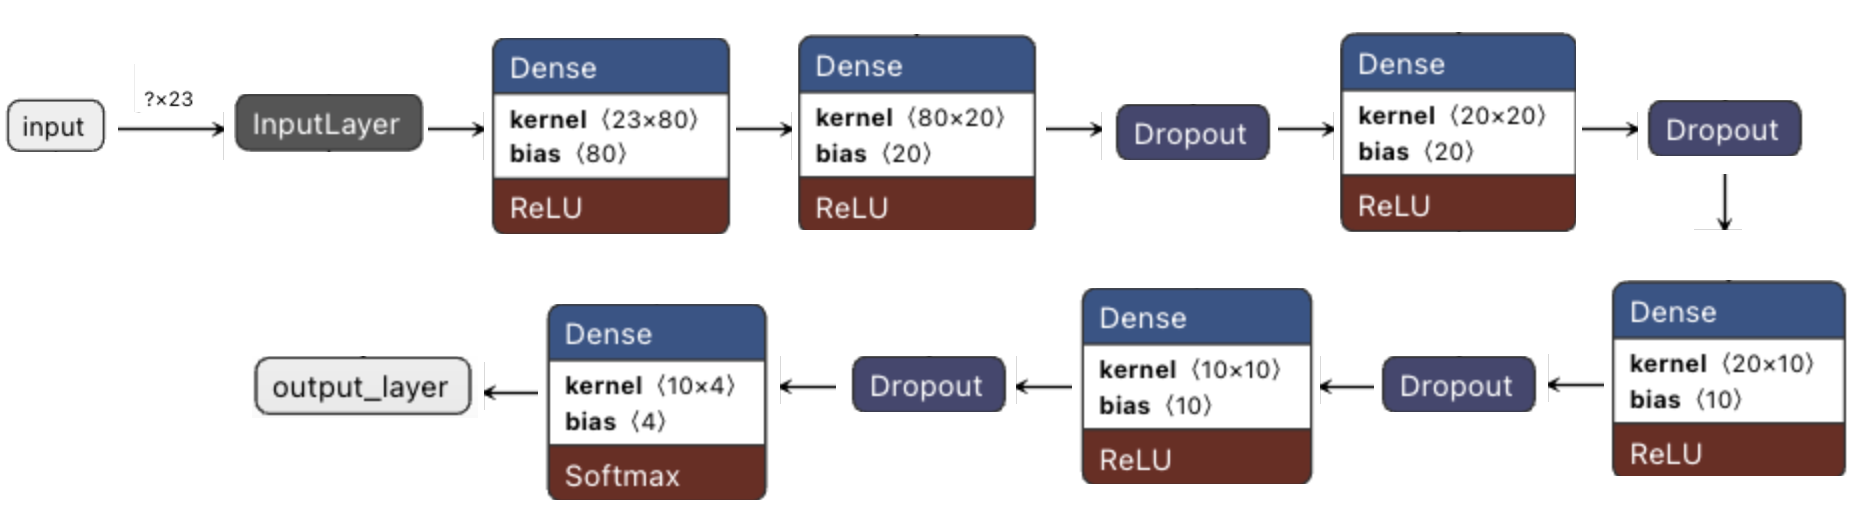
\includegraphics[scale=0.3]{model.png} 
% \caption{Caption1}
% \label{fig:subim1}
% \end{subfigure}
% \begin{subfigure}{0.5\textwidth}
% \hspace*{3cm}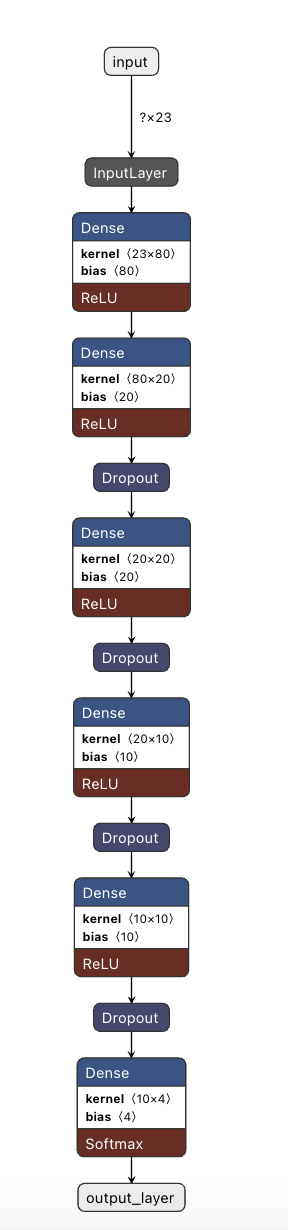
\includegraphics[scale=0.7]{architecture.png}
% \caption{Architecture of DNN model}
% \label{fig:subim2}
% \end{subfigure}
% \caption{Caption for this figure with two images}
% \label{fig:image2}
% \end{figure}





\section{Results}
In this project, we are mainly interested in the following aspects of this dataset: 1. The distribution and summary statistics of the song features('danceability', 'energy', 'key', 'loudness',...) in each playlist associated with one of the four moods(angry, chilling, happy, depression). We’d like to know whether there is a significant distinction among features of songs with different moods. 2. We will explore the possible correlations among numerical features of songs to detect any potential relationships between certain variables. 3. The last, and the most important task of this project is to implement models to classify songs with mood labels and find the model that has the best performance. \\
\\
We first grouped the dataset based on the moods and computed the summary statistics of all the song features. The results are mostly as expected. ‘Happy’ songs have the highest danceability and valence on average. ‘Angry’ songs have the highest energy, loudness, speechiness, liveness, tempo and lowest acousticness on average. ‘Chilling’ songs have the highest instrumentalness on average. ‘Depression’ songs have the lowest danceability, energy, loudness, speechiness, instrumentalness, liveness, valence, tempo and highest acousticness and duration\_ms. The key, mode and time\_signiture distributions of songs with all moods don’t differ much. In addition, we found a strong negative correlation between the acousticness and energy feature, and a moderate negative correlation between the acousticness and loudness feature of songs. \\
\\
We then ran our models on the training and test data. For the SVM model in particular, we split the features into continuous and categorical subsets and fit the model separately. The result in Table 1 shows that, for continuous data, using the rbf kernel gives us the highest accuracy rate($0.546667$) while the sigmoid kernel gives us the lowest accuracy rate($0.396667$). For categorical data, using linear kernel gives us the highest accuracy rate($0.2825$) while the sigmoid kernel gives us the lowest accuracy rate($0.246667$). We also ran the model on a selected smaller subset of the continuous features("danceability","energy","loudness","acousticness","valence"). Again, using the rbf kernel gives the highest accuracy rate($0.53$) while the sigmoid kernel gives the lowest accuracy rate($0.405$). Then, we fit Decision Tree,  Random Forest and Linear Discriminant Analysis models on the combined training data. The result indicates that the Random Forest model performs the best($0.575$). Decision Tree model has a slightly worse performance($0.433333$)\\
\\
Lastly, we implemented the Deep Neural Network model. We first split the song features into continuous and categorical subsets again, and performed principal component analysis to reduce the dimensionality of the input data and increase computation efficiency. Then, we implemented the Deep Neural Network model with ‘ReLu’ as activation function. According to the result in Table 2, for continuous data with PCA, 'Adadelta' optimizer gives us the highest accuracy rate($0.5150$) while 'RMSprop' gives us the lowest accuracy rate($0.373800$). We then repeat the procedure on the original continuous data. Again, 'Adadelta' optimizer gives us the highest accuracy rate($0.546200$) while 'Adam' gives us the lowest accuracy rate($0.515000$). We then test the model on the selected subset of features. 'RMSprop' optimizer gives us the highest accuracy rate($0.515000$) while 'Adam' gives us the lowest accuracy rate($0.455000$). For the combined data with pca, 'Adagrad' optimizer gives us the highest accuracy rate($0.496300$) while 'RMSprop' gives us the lowest accuracy rate($0.451200$). For the combined data without pca,  'Adadelta' optimizer gives us the highest accuracy rate($0.437500$) while 'SGD' gives us the lowest accuracy rate($0.242500$).

\begin{table}
\caption{Accuracy rates of SVM model with different kernal functions/datasets}
\centering
\begin{tabular}{lrrr}
\hline
\toprule
 & continuous features & categorical features & selected continuous features \\
\midrule
\hline
linear & 0.531667 & 0.282500 & 0.500000 \\
ploy & 0.517500 & 0.272500 & 0.505000 \\
rbf & 0.546667 & 0.267500 & 0.530000 \\
sigmoid & 0.396667 & 0.246667 & 0.405000 \\
\bottomrule
\hline
\end{tabular}
\end{table}

\begin{table}
\caption{Accuracy rates of DNN model with different optimizers/datasets}
\centering
\begin{tabular}{lrrrrr}
\hline
\toprule
 & Adadelta & Adagrad & Adam & RMSprop & SGD \\
\midrule
\hline
continuous features with pca & 0.515000 & 0.493800 & 0.503800 & 0.373800 & 0.513800 \\
continuous features without pca & 0.507500 & 0.522500 & 0.442500 & 0.420000 & 0.227500 \\
selected combined features with pca & 0.475000 & 0.503800 & 0.455000 & 0.515000 & 0.480000 \\
selected combined features without pca & 0.475000 & 0.503800 & 0.455000 & 0.515000 & 0.480000 \\
combined features with pca & 0.480000 & 0.496300 & 0.477500 & 0.451200 & 0.493800 \\
combined features without pca & 0.437500 & 0.261200 & 0.242500 & 0.392500 & 0.401300 \\
\bottomrule
\hline
\end{tabular}
\end{table}

\section{Conclusion}
In this study, we investigated the classification of music based on mood using various machine learning techniques. Our goal was to explore the potential of efficiently categorizing music and contributing to developing personalized music recommendation systems. \\

Through data preprocessing, including normalization, outlier removal, and denoising, we prepared the dataset obtained from the Spotify API. Subsequently, we employed different classification methods, including kernel-based Support Vector Machines (SVM), Deep Neural Networks (DNN), Decision Trees, Random Forests, and Linear Discriminant Analysis. \\

Our results revealed that while not all methods achieved high accuracy, specific approaches performed relatively better. The SVM model, specifically with the 'rbf' kernel, demonstrated the highest accuracy for continuous data, while the 'linear' kernel yielded the best results for categorical data.
Additionally, the random forest model outperformed the decision tree model. In the case of the DNN model, the 'Adadelta' optimizer exhibited the highest accuracy for both PCA-reduced and original continuous data.\\

In conclusion, our study highlights the challenges and potential of music mood classification using machine learning techniques. The SVM model with the 'rbf' kernel and the random forest model emerged as promising approaches in accurately categorizing music based on mood. These findings contribute to the advancement of personalized music recommendation systems, benefiting users in discovering music that aligns with their desired mood. Future research can focus on further improving classification accuracy, exploring additional features, and considering the interpretability of the models for a more comprehensive understanding of music mood classification.

\section{Discussion}
One of the significant limitations of our study was the overall lower accuracy than anticipated, despite specific approaches demonstrating relatively higher accuracy. Upon reflection, the main factor that significantly impacted our results was the potential overlap in classification due to subjective interpretations when categorizing music based on mood. As music classification involves subjective elements, it becomes challenging to establish precise definitions. Although we utilized pre-classified mood playlists from Spotify, these playlists likely contained overlapping elements. Moreover, we proceeded with the project assuming perfect classification, contributing to the lower overall accuracy. We are confident that utilizing more accurately classified playlists would have yielded higher accuracy in our study.

\section*{Reference}
\begin{enumerate}
\item Web API | Spotify for Developers. (n.d.-a). https://developer.spotify.com/documentation/web-api 
\item Netron. (2023, June 10). https://netron.app/ 
\item Brownlee, J. (2022, August 2). Tensorflow 2 tutorial: Get started in deep learning with tf.keras. MachineLearningMastery.com. https://machinelearningmastery.com/tensorflow-tutorial-deep-learning-with-tf-keras/ 
\item Features description. https://developer.spotify.com/documentation/web-api/reference/get-several-audio-features
\end{enumerate}


% \section*{Appendix}
% \subsection*{Continuous data}
% \begin{enumerate}
%     \item \textbf{danceability:} Danceability describes how suitable a track is for dancing based on a combination of musical elements including tempo, rhythm stability, beat strength, and overall regularity. A value of 0.0 is least danceable and 1.0 is most danceable.
%     \item \textbf{energy:} Energy is a measure from 0.0 to 1.0 and represents a perceptual measure of intensity and activity. Typically, energetic tracks feel fast, loud, and noisy.
%     \item \textbf{loudness:} The overall loudness of a track in decibels (dB). Loudness values are averaged across the entire track and are useful for comparing relative loudness of tracks. 
%     \item \textbf{speechiness:} Speechiness detects the presence of spoken words in a track. The more exclusively speech-like the recording (e.g. talk show, audio book, poetry), the closer to 1.0 the attribute value.
%     \item \textbf{acousticness:} A confidence measure from 0.0 to 1.0 of whether the track is acoustic. 1.0 represents high confidence the track is acoustic
%     \item \textbf{instrumentalness:} Predicts whether a track contains no vocals. "Ooh" and "aah" sounds are treated as instrumental in this context. Rap or spoken word tracks are clearly "vocal". The closer the instrumentalness value is to 1.0, the greater likelihood the track contains no vocal content. 
%     \item \textbf{liveness:} Detects the presence of an audience in the recording. Higher liveness values represent an increased probability that the track was performed live. A value above 0.8 provides strong likelihood that the track is live.
%     \item \textbf{valence:} A measure from 0.0 to 1.0 describing the musical positiveness conveyed by a track. Tracks with high valence sound more positive (e.g. happy, cheerful, euphoric), while tracks with low valence sound more negative (e.g. sad, depressed, angry).
%     \item \textbf{tempo:} The overall estimated tempo of a track in beats per minute (BPM). In musical terminology, tempo is the speed or pace of a given piece and derives directly from the average beat duration.
% \end{enumerate}

% \subsection*{Categorical features}
% \begin{enumerate}
%     \item \textbf{key:} The key the track is in. Integers map to pitches using standard Pitch Class notation. E.g. 0 = C, 1 = C♯/D♭, 2 = D, and so on. If no key was detected, the value is -1. 
%     \item \textbf{mode:} The key the track is in. Integers map to pitches using standard Pitch Class notation. E.g. 0 = C, 1 = C♯/D♭, 2 = D, and so on. If no key was detected, the value is -1.
%     \item \textbf{time signature:} An estimated time signature. The time signature (meter) is a notational convention to specify how many beats are in each bar (or measure). 
% \end{enumerate}




\printbibliography

\end{document}
